\documentclass[a4paper, 10pt, twoside]{article}

\usepackage[top=1in, bottom=1in, left=1in, right=1in]{geometry}
\usepackage[utf8]{inputenc}
\usepackage[spanish, es-ucroman, es-noquoting]{babel}
\usepackage{setspace}
\usepackage{fancyhdr}
\usepackage{lastpage}
\usepackage{amsmath}
\usepackage{amsfonts}
\usepackage{amsthm}
\usepackage{graphicx}
\usepackage{float}
\usepackage{enumitem} % Provee macro \setlist
\usepackage{tabularx}
\usepackage{multirow}
\usepackage{hyperref}
\usepackage{multicol}
\usepackage{verbatim}
\usepackage{listings}
\usepackage[toc, page]{appendix}
\usepackage{color}


%%%%%%%%%% Configuración de Fancyhdr - Inicio %%%%%%%%%%
\pagestyle{fancy}
\thispagestyle{fancy}
\lhead{Trabajo Práctico 2 · Ingeniería de Software I}
\rhead{Aboy Solanes · Almansi · Canay · Contrufo · Decroix}
\renewcommand{\footrulewidth}{0.4pt}
\cfoot{\thepage /\pageref{LastPage}}

\fancypagestyle{caratula} {
   \fancyhf{}
   \cfoot{\thepage /\pageref{LastPage}}
   \renewcommand{\headrulewidth}{0pt}
   \renewcommand{\footrulewidth}{0pt}
}
%%%%%%%%%% Configuración de Fancyhdr - Fin %%%%%%%%%%


%%%%%%%%%% Miscelánea - Inicio %%%%%%%%%%
% Evita que el documento se estire verticalmente para ocupar el espacio vacío
% en cada página.
\raggedbottom

% Deshabilita sangría en la primer línea de un párrafo.
\setlength{\parindent}{0em}

% Separación entre párrafos.
\setlength{\parskip}{0.5em}

% Separación entre elementos de listas.
\setlist{itemsep=0.5em}

% Asigna la traducción de la palabra 'Appendices'.
\renewcommand{\appendixtocname}{Apéndices}
\renewcommand{\appendixpagename}{Apéndices}
%%%%%%%%%% Miscelánea - Fin %%%%%%%%%%


%%%%%%%%%% Insertar diagrama - Inicio %%%%%%%%%%
\newcommand{\diagramav}[1]{%
  \includegraphics[type=pdf,ext=.pdf,read=.pdf,width=16cm]{diagramas/#1}%
}

\newcommand{\diagramavtrim}[2]{%
  \includegraphics[type=pdf,ext=.pdf,read=.pdf,width=16cm,trim=0 #2 0 0,clip]{diagramas/#1}%
}

\newcommand{\diagramah}[1]{%
  \includegraphics[type=pdf,ext=.pdf,read=.pdf,height=16cm,angle=90]{diagramas/#1}%
}
%%%%%%%%%% Insertar diagrama - Fin %%%%%%%%%%


%%%%%%%%%% Macros para Casos de Uso - Inicio %%%%%%%%%%
\newcounter{usecasecounter}
\newcounter{usecasealtcounter}
\newcounter{nroCU}
\setcounter{nroCU}{0}

\newcommand{\ucname}[1]{\renewcommand{\givenucname}{#1}}
\newcommand{\ucpre}[1]{\renewcommand{\givenucpre}{#1}}
\newcommand{\ucpost}[1]{\renewcommand{\givenucpost}{#1}}
\newcommand{\ucactor}[1]{\renewcommand{\givenucactor}{#1}}
\newcommand{\givenucname}{REQUIRED!}
\newcommand{\givenucpre}{REQUIRED!}
\newcommand{\givenucpost}{REQUIRED!}
\newcommand{\givenucactor}{REQUIRED!}

\newenvironment{usecase}
  {}{
    \stepcounter{nroCU}
    \textbf{Caso de uso \arabic{nroCU}: }\givenucname \\
    \textbf{Pre: }\givenucpre \\
    \textbf{Post: }\givenucpost \\
    \textbf{Actores: }\givenucactor
  }

\newenvironment{usecasesteps}
  {
    \setcounter{usecasecounter}{0}
    \setcounter{usecasealtcounter}{0}

    \tabularx{\textwidth}{|l|X|}
    \hline
    Curso normal & Curso alternativo \\
    \hline
    \hline
  }{
    \endtabularx
    \vspace{\parskip}
  }

\newcommand{\ucstep}[2]{
  \stepcounter{usecasecounter}%
  \parbox[t]{7.5cm}{
    \makebox[2ex][l]{\arabic{usecasecounter}.}
    #1\phantom{p}
  }
  &
  \parbox[t]{7.5cm}{
    \setcounter{usecasealtcounter}{0}
    #2\phantom{p}
  } \\
  \hline
}

\newcommand{\ucalt}[1]{
  \stepcounter{usecasealtcounter}
  \makebox[4ex][l]{\arabic{usecasecounter}.\arabic{usecasealtcounter}.}
  #1
}
%%%%%%%%%% Macros para Casos de Uso - Fin %%%%%%%%%%


%%%%%%%%%% Macro para OCL - Inicio %%%%%%%%%%%%
\newenvironment{ocl}[1]
  {
    \textbf{#1}
    \verbatim
  }{
    \endverbatim
  }
%%%%%%%%%% Macro para OCL - Fin %%%%%%%%%%%%


\begin{document}


%%%%%%%%%%%%%%%%%%%%%%%%%%%%%%%%%%%%%%%%%%%%%%%%%%%%%%%%%%%%%%%%%%%%%%%%%%%%%%%
%% Carátula                                                                  %%
%%%%%%%%%%%%%%%%%%%%%%%%%%%%%%%%%%%%%%%%%%%%%%%%%%%%%%%%%%%%%%%%%%%%%%%%%%%%%%%


\thispagestyle{caratula}

\begin{center}


\includegraphics[height=2cm]{DC.png} 
\hfill

\includegraphics[height=2cm]{UBA.jpg} 

\vspace{2cm}

Departamento de Computación,\\
Facultad de Ciencias Exactas y Naturales,\\
Universidad de Buenos Aires

\vspace{4cm}

\begin{Huge}
Trabajo Práctico 2
\end{Huge}

\vspace{0.5cm}

\begin{Large}
Ingeniería de Software I
\end{Large}

\vspace{1cm}

Segundo Cuatrimestre de 2014

\vspace{4cm}

\begin{tabular}{|c|c|c|}
\hline
Apellido y Nombre & LU & E-mail\\
\hline
Santiago Aboy Solanes & 175/12 & santiaboy2@hotmail.com \\
Emilio Almansi & 674/12 & ealmansi@gmail.com \\
Federico Canay & 250/12 & fcanay@hotmail.com \\
Maximiliano Contrufo & 336/12 & maxicontru@gmail.com  \\
Facundo Decroix & 842/11 & fndecroix92@hotmail.com \\
\hline
\end{tabular}

\end{center}

\newpage


%%%%%%%%%%%%%%%%%%%%%%%%%%%%%%%%%%%%%%%%%%%%%%%%%%%%%%%%%%%%%%%%%%%%%%%%%%%%%%%
%% Índice                                                                    %%
%%%%%%%%%%%%%%%%%%%%%%%%%%%%%%%%%%%%%%%%%%%%%%%%%%%%%%%%%%%%%%%%%%%%%%%%%%%%%%%


\tableofcontents

\newpage


%%%%%%%%%%%%%%%%%%%%%%%%%%%%%%%%%%%%%%%%%%%%%%%%%%%%%%%%%%%%%%%%%%%%%%%%%%%%%%%
%% Introducción                                                              %%
%%%%%%%%%%%%%%%%%%%%%%%%%%%%%%%%%%%%%%%%%%%%%%%%%%%%%%%%%%%%%%%%%%%%%%%%%%%%%%%


\section{Introducción}

En el siguiente informe, vamos a profundizar acerca del sistema propuesto a TecnoTaxi. Para ello, vamos a utilizar un diagrama de modelo conceptual y mostraremos mediante la utilización de OCL los invariantes que se aplican sobre el mismo. Por otro lado, vamos a utilizar diagramas del model de casos de uso para mostrar la interacción de los usuarios con el sistema. Finalmente, vamos a utilizar diagramas de actividad para detallar acerca de interacciones específicas.

Además, vamos a garantizar la \emph{trazabilidad} transversalmente entre los distintos modelos creados.

%%%%%%%%%%%%%%%%%%%%%%%%%%%%%%%%%%%%%%%%%%%%%%%%%%%%%%%%%%%%%%%%%%%%%%%%%%%%%%%
%% Desarrollo                                                                %%
%%%%%%%%%%%%%%%%%%%%%%%%%%%%%%%%%%%%%%%%%%%%%%%%%%%%%%%%%%%%%%%%%%%%%%%%%%%%%%%


\section{Decisiones tomadas}

Incluimos en Trabajo Práctico 1 dentro del Trabajo Práctico 2 porque creemos que el Trabajo Práctico 2 incluye al Trabajo Práctico 1.

% Debido a que la continuidad del proyecto requería de la elección de una de las alternativas propuestas anteriormente para la distribución de bicicletas en hora pico, elegimos la propuesta de que las distribuciones se realicen de manera automática utilizando los datos estadísticos recaudados por el sistema.
% 
% Esta elección se debe a que la distribución automática propone una manera más simple y precisa, ya que no se requiere de nadie calculando o decidiendo para cada estación, que cantidad de bicicletas le toca a cada una, permitiendo así, un mejor uso de los recursos disponibles.


%%%%%%%%%%%%%%%%%%%%%%%%%%%%%%%%%%%%%%%%%%%%%%%%%%%%%%%%%%%%%%%%%%%%%%%%%%%%%%%
%% Diferencias con especificaciones anteriores                               %%
%%%%%%%%%%%%%%%%%%%%%%%%%%%%%%%%%%%%%%%%%%%%%%%%%%%%%%%%%%%%%%%%%%%%%%%%%%%%%%%


% \section{Diferencias con especificaciones anteriores}

% A continuación listaremos algunos cambios realizados a la solución propuesta con respecto a las especificaciones presentadas previamente.

% \begin{itemize}
%  \item Cuando el empleado de estación consulta el monto de una multa que debe ser pagada por un usuario, ingresa en el sistema el DNI de este último. Aquí agregamos que el sistema valide ese DNI e indique por pantalla que hubo un error si este no pertenecía a ningún usuario registrado.
%  \item Las operaciones de registro (no de consulta) que pueden ser realizadas a través de un radio requieren que un empleado de otra estación ingrese los datos al sistema. Para esto, fue necesario agregar la posibilidad de que el empleado de estación ingrese el ID de ésta para realizar dichas operaciones y así permitir que ingrese datos de otra estación. Además se agregó una validación de ese ID (debe corresponder a una estación registrada en el sistema).
%  \item Cuando sale o llega un camión con bicicletas, el empleado de estación registra los IDs de las bicicletas que envía o recibe. Las bicicletas que llegan deben coincidir con las que salieron. Pero podría suceder que en la estación origen se informaran ciertas bicicletas pero se enviaran otras. Para poder corregir este error, debimos agregar:
%  \begin{itemize}
%   \item Las órdenes de transporte de bicicletas tienen un ID para poder identificar qué envío es el que se está informando en la estación destino, y así asociarlo con la estación origen. Este ID  es validado (debe corresponder a una orden de transporte registrada).
%   \item Agregamos una validación de IDs de bicicletas ingresadas en la estación destino para poder detectar los errores e informarlos.
%  \end{itemize}
%  \item Cuando el gobierno registra bicicletas nuevas en el sistema, puede hacerlo por cantidad (antes sólo podía ingresar de a una). Además el sistema le muestra los IDs asignados a las bicicletas nuevas para que el personal del gobierno pueda grabarlos en las bicicletas y se indica también la estación inicial de las bicicletas. Por último, el personal del gobierno se encarga ahora de la distribución de las nuevas bicicletas, eliminando el requerimiento de enviar un mail a la empresa de transporte.
%  \item Cuando el gobierno ingresa una nueva estación al sistema, agregamos la validación del nombre y dirección, para evitar estaciones duplicadas.
%  \item Cuando el gobierno elimina bicicletas del sistema, agregamos la validación del ID de la bicicleta (debe existir).
%  \item Cuando el gobierno consulta las estadísticas, ademas de poder consultar la demanda de cada estación, ahora puede:
%  \begin{itemize}
%   \item Consultar que usuarios estan registrados.
%   \item Consultar que usuarios estan penalizados.
%   \item Averiguar cuales son las 5 estaciones con más solicitudes en hora pico.
%   \item Averiguar cuales son las 5 estaciones con más solicitudes fuera de hora pico.
%  \end{itemize}
%  \item El gobierno ahora puede invalidar penalizaciones de determinado usuario.
%  \item Cuando un usuario no devuelve la bicicleta por más de 24hs se informa al gobierno. Pero si la bicicleta es devuelta, agregamos un nuevo aviso al gobierno indicando esto.
%  \item El stock en una estación ya no se consulta a voluntad, si no que es calculado durante el ingreso de la solicitud de bicicleta (ver {\bf CU 8}).
% \end{itemize}

\section{Escenarios hipotéticos}

Los siguientes escenarios ilustran de manera informal situaciones representativas del funcionamiento esperado del sistema.

\subsection{Escenario 1}

Alicia necesita viajar hasta el consultorio de su dentista y elige la moderna empresa TecnoTaxi para solicitar un taxi. Como ella está al día en cuestiones tecnológicas, tiene instalada la aplicación de la empresa en su smartphone y desea realizar la solicitud mediante la misma.

Alicia inicia el proceso de solicitud en la aplicación, ingresando la dirección de origen del viaje, la dirección destino y sus preferencias: un auto moderno. El sistema le muestra mediante la aplicación una lista de opciones de diferentes taxistas que cumplen su pedido y ella elige a Florencia, que maneja un Chevrolet último modelo.

\subsection{Escenario 2}

Omar pidió un taxi para las 17:00hs, para ir a visitar a su suegra. Afortunadamente, ella lo llama para postergar el encuentro. Omar usa su teléfono para avisar a TecnoTaxi y cancelar su viaje.

\subsection{Escenario 3}

Micaela realizó un viaje durante el cual el conductor le realizó múltiples insinuaciones. Ni bien terminó su viaje, dio una calificación de una estrella al conductor y publicó un comentario para que no le pase a nadie más.

\subsection{Escenario 4}

Cada vez que Lucas viaja con su taxista preferido, Roberto, llega a su destino con una sonrisa en su cara. Roberto es un gran comediante amateur. Lucas decide calificar a Roberto positivamente para que todos sepan lo buena persona que es.

\subsection{Escenario 5}

Alfredo desea ir a visitar a su tía, que vive en Boedo. Él es un pasajero usual de TecnoTaxi, por lo que tiene ya descargada en su smartphone la aplicación móvil de viajes. Al abrir la aplicación, la misma le indica que no se puede encontrar una conexión a internet, por lo que deberá comunicarse por otros medios, sugiriendo la página web de la empresa y el número de teléfono para comunicarse por vía telefónica. Alfredo se dirige entonces a su computadora para solicitar el taxi vía web. Al abrir el navegador web, su página de inicio no carga correctamente. Sorprendido, Alfredo tipea la dirección de la página web indicada por la aplicación, pero su computadora tampoco logra cargarla: no tiene acceso a internet. Indignado por el pésimo servicio de internet que brindan tanto el servidor de internet que utiliza en su casa como el del celular, Alfredo decide hacer su pedido de viaje por teléfono. Llama a la línea telefónica de la empresa de taxis y es atendido por una cordial operadora, y realiza el pedido por 
este medio.

\subsection{Escenario 6}

Ronaldo va a su masajista todos los martes a las 15:00hs. Necesita un taxi para llegar a horario y no perder la sesión de masajes. Ronaldo llama a TecnoTaxi y programa un viaje de rutina para las 14:30hs de todos los martes. Desde ese momento y hasta el día presente, Ronaldo no perdió ninguna sesión de masajes.


%%%%%%%%%%%%%%%%%%%%%%%%%%%%%%%%%%%%%%%%%%%%%%%%%%%%%%%%%%%%%%%%%%%%%%%%%%%%%%%
%% Desarrollo                                                                %%
%%%%%%%%%%%%%%%%%%%%%%%%%%%%%%%%%%%%%%%%%%%%%%%%%%%%%%%%%%%%%%%%%%%%%%%%%%%%%%%


\section{Desarrollo}

\subsection{Requerimientos}

\begin{enumerate}
 \item Brindar a los usuarios esperando un taxi la información de donde se encuentra el mismo y cual es el tiempo de demora.
 \item Poder calificar los viajes, para que otros usuarios puedan elegir no viajar con determinado chofer.
 \item Que el cliente pueda elegir el coche con el que viajar.
 \item Que a los taxistas solo le ofrezca la operadora viajes dentro de su alcance.
 \item Brindar al usuario una opción para cancelar el viaje.
 \item Que los pasajeros puedan solicitar un viaje vía web o móvil.
 \item Seguir aportando servicio a los pasajeros sin acceso a Internet o a la tecnología.
 \item Que los pasajeros puedan planificar viajes de rutina.
 \item Automatizar la asistencia al pasajero en la elección de auto/chofer.
 \item Proveer un conjunto de estadísticas para los directivos.
\end{enumerate}

\subsection{Acerca de Trazabilidad}

Para garantizar la trazabilidad entre los en este trabajo práctico, decidimos dividirla en las distintas secciones. Así, por ejemplo, la trazabilidad correspondiente a los casos de uso, está presente en la sección homónima.

Por otro lado, para que el trabajo práctico tenga mayor claridad, vamos a enumerar algunas cuestiones generales acerca de la trazabilidad. Estas cuestiones son válidas para todo el trabajo práctico, a menos que indiquemos lo contrario en la sección correspondiente:

\begin{itemize}
	\item Cuando hablamos de Taxista, nos vamos a referir al empleado de la empresa que maneja el taxi.
	\item Cuando hablamos del Sistema, nos referimos al sistema que vamos a construir.
	\item Cuando hablamos de clientes, nos referimos a los clientes de la empresa.
	\item Cuando hablamos de directivos, nos referimos a los empleados de la empresa encargados de dirigirla.
	\item Cuando hablamos de aplicación web o móvil nos referimos a la aplicación web o móvil (respectivamente) que no vamos a construir nosotros. Construir estas apliaciones queda por fuera de nuestro sistema, como se puede observar en el Diagrama de Contexto.
\end{itemize}



%%%%%%%%%%%%%%%%%%%%%%%%%%%%%%%%%%%%%%%%%%%%%%%%%%%%%%%%%%%%%%%%%%%%%%%%%%%%%%%
%% Diagrama de Contexto                                                      %%
%%%%%%%%%%%%%%%%%%%%%%%%%%%%%%%%%%%%%%%%%%%%%%%%%%%%%%%%%%%%%%%%%%%%%%%%%%%%%%%

\section{Diagrama de contexto}

  \begin{figure}[H]
    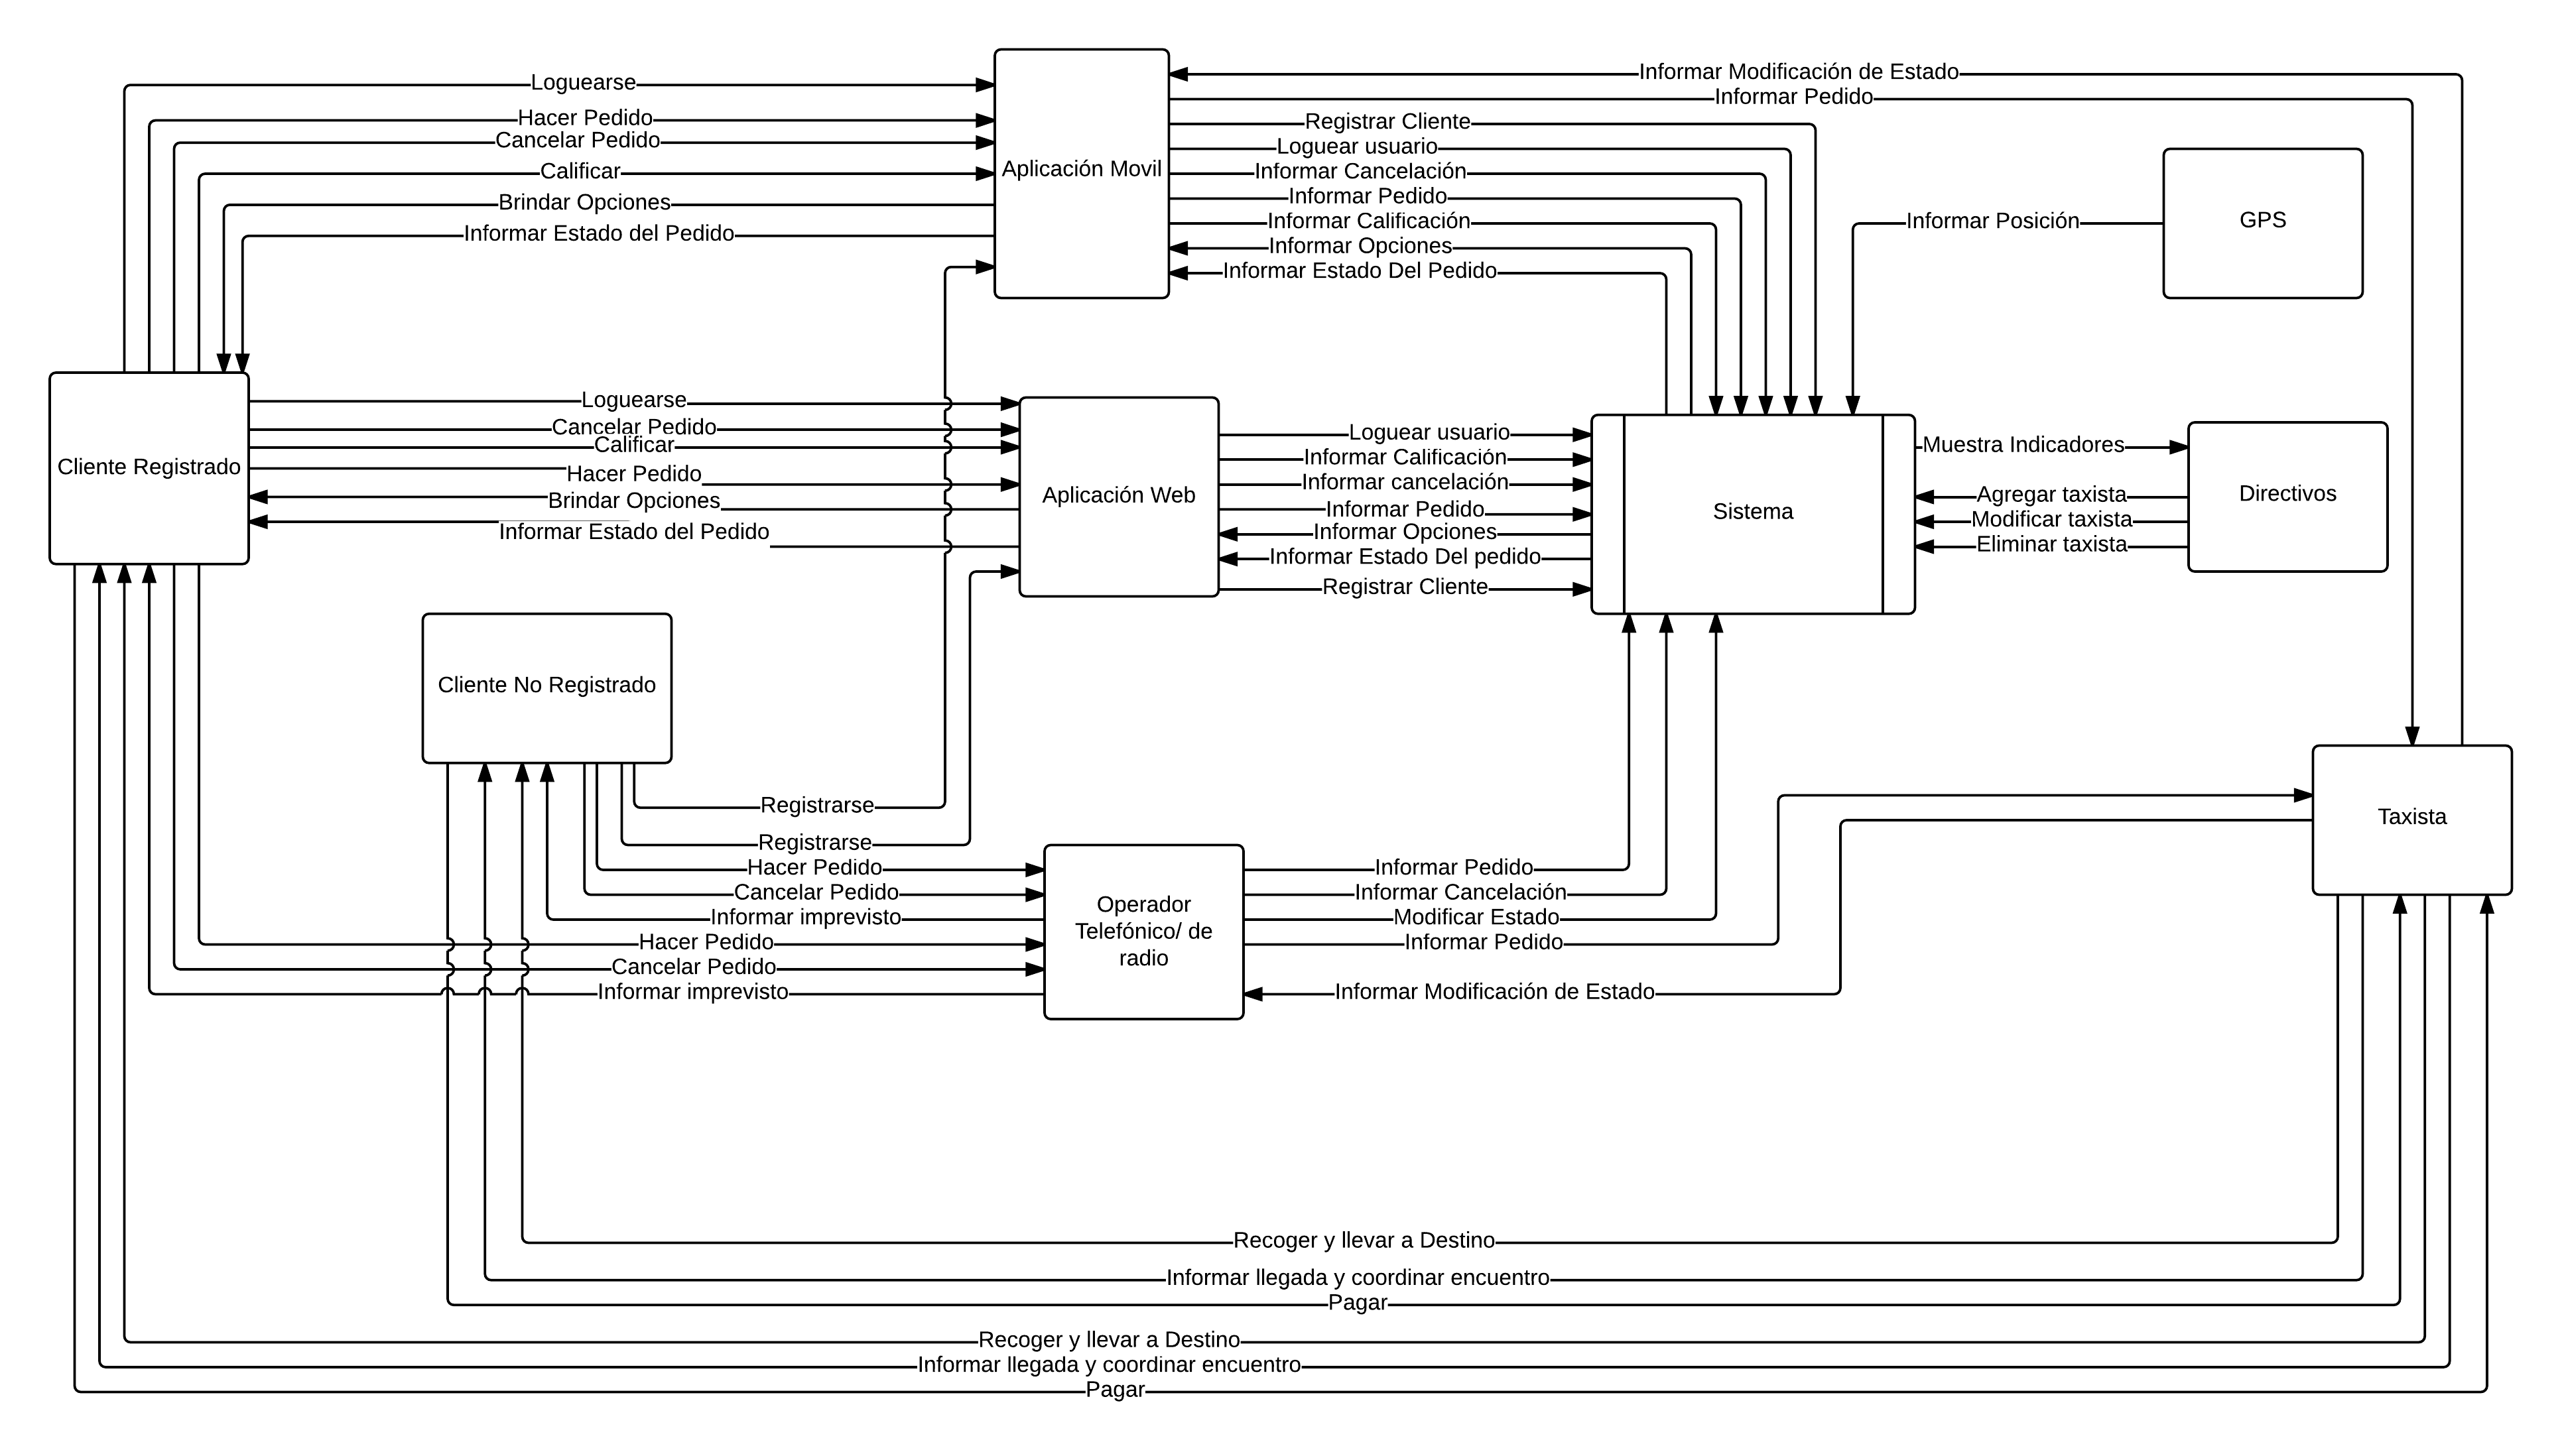
\includegraphics[height=15cm,angle=90]{diagramas/contexto.png}
  \end{figure}

\subsection{Actores}

A continuación, vamos a explicar los distintos actores que están presentes en nuestro diagrama de contexto.

  \begin{enumerate}
    \item \textbf{Sistema:} El sistema a crear.
    \item \textbf{Aplicación Móvil:} Aplicación móvil con la cual los usuarios pueden pedir taxis, calificar taxistas, etc. Esta aplicación es externa a nuestro sistema.
    \item \textbf{Aplicación Web:} Aplicación web con la cual los usuarios pueden pedir taxis, calificar taxistas, etc. Esta aplicación es externa a nuestro sistema.
    \item \textbf{Operador Telefónico/ de radio:} Empleado de la empresa encargado de atender teléfonos, y hablar con taxistas para coordinar viajes.
    \item \textbf{Cliente No Registrado:} Cualquier persona que se comunique vía telefónica, sin importar si tiene un usuario registrado en el sistema o no.
    \item \textbf{Cliente Registrado:} Cualquier persona que se haya registrado previamente en el sistema. Registrando un nombre de usuario y una contraseña.
    \item \textbf{Directivos:} Empleados de la empresa encargados de dirigir la misma.
    \item \textbf{Taxista:} Un empleado de la empresa que maneja taxis.
    \item \textbf{GPS:} Sistema de navegación y localización mediante satélites.
  \end{enumerate}

\subsection{Fenómenos destacados}

A continuación, vamos a enumerar y explicar algunos fenómenos que creemos que vale la pena aclarar.

   \begin{enumerate}
     \item \textbf{Informar Modificación de Estado:} Por Informar Modificación de Estado nos referimos a que el taxista informa si surgió un contratiempo, como por ejemplo que pinchó una goma.
     \item \textbf{Hacer Pedido:} Por Hacer Pedido nos referimos a que el cliente indica desde donde, a donde quiere ir y cuáles son sus preferencias (si las tiene).
     \item \textbf{Brindar Opciones:} Por Brindar Opciones nos referimos a que las aplicaciones le indican al cliente cuáles son las mejores opciones de taxistas dado su pedido.
     \item \textbf{Informar llegada y coordinar encuentro:} Por Informar llegada y coordinar encuentro nos referimos a que el taxista le avisa al cliente que llegó a la dirección coordenada para empezar el viaje.
     \item \textbf{Calificar:} Por Calificar nos referimos a que el cliente califica a un cierto taxista, con una cierta cantidad de estrellas (1-5).
  \end{enumerate}
 
 \subsection{Aclaraciones}
 
 Cabe resaltar que el optar por dejar la Aplicación M\'ovil y la Aplicación Web por fuera del sistema, deja de ser parte del producto que vamos a realizar y pasa a hacer algo que se supone que se consigue.
 
\newpage

%%%%%%%%%%%%%%%%%%%%%%%%%%%%%%%%%%%%%%%%%%%%%%%%%%%%%%%%%%%%%%%%%%%%%%%%%%%%%%%
%% Modelo de Objetivos                                                       %%
%%%%%%%%%%%%%%%%%%%%%%%%%%%%%%%%%%%%%%%%%%%%%%%%%%%%%%%%%%%%%%%%%%%%%%%%%%%%%%%


\section{Modelo de objetivos}

%TODO agregar el diagrama en si

\newpage

\subsection{Objetivos de alto nivel}

En esta sección vamos a explicar un poco los objetivos de alto nivel, y por qué están en esas posiciones en el diagrama.

\begin{itemize}

\item \textbf{Lograr [Incrementar Ganancias]}: Con esto, nos referimos al objetivo primordial de las empresas con fines de lucro: ganar dinero.
\end{itemize}
Este objetivo, se desglosa en objetivos más pequeños:
\begin{itemize}

\item \textbf{Lograr [Incrementar Ingresos]}: Incrementar ingresos ayuda a desestancar la facturación ya que efectivamente la empresa tiene más dinero.

\item \textbf{Lograr [Reducir costos]}: La contracara de incrementar ingresos, es reducir los egresos o costos. Claramente, gastar menos dinero ayuda a incrementar ganancias.

\item \textbf{Lograr [Proveer estadísticas e indicadores]}: Con esto nos referimos a proveer estadísticas como por ejemplo calificación de taxistas.

\item \textbf{Conocer estadísticas acerca del ambiente del trabajo, permite aumentar las ganancias}: Al conocer las estadísticas del ambiente del trabajo, puedo obtener un mejor conocimiento del medio. Esto permite podes aprovechar mejor el capital, incurriendo en mayores ingresos y/o menores ingresos.

\end{itemize}

Creemos que estos últimos objetivos, en conjunto, logran que efectivamente se incrementen las ganancias de la empresa.

\subsection{Objetivos blandos}

En esta sección vamos a hablar de los \emph{o-refinamientos} del diagrama de objetivos y de cuáles son los objetivos blandos que utilizamos para compararlos.

\begin{itemize}
\item Lograr darse a conocer

  De este objetivo surge un \emph{o-refinamiento} que deriva en los siguientes objetivos:
  \begin{enumerate}
    \item Lograr armar campaña publicitaria
    \item Lograr estar presente en las redes sociales
  \end{enumerate}
	
  Para ponderar estas opciones del \emph{o-refinamiento} consideramos los siguientes objetivos blandos:
  \begin{enumerate}
    \item Efectividad en el corto plazo (menos de 3 meses)
      
      En este caso ambos objetivos aportan positivamente. Sin embargo nos parece que el primero es aún más efectivo a corto plazo que el segundo, ya que consideramos que una campaña publicitaria tiene un alcance más veloz que el de las redes sociales.

    \item Disminuir costo en el corto plazo (menos de 3 meses) %mediano plazo no hay diferencias asi que no hay objetivos blandos al respecto
      
      Creemos que ambos objetivos aportan negativamente a este objetivo ya que involucran gastos a la empresa. Sin embargo creemos que el primer objetivo es el que va más en contra de este objetivo ya que es más costosa una campaña publicitaria que estar presente en redes sociales.
    
    \item Disminuir costo en el largo plazo (mas de 1 año)
      
      Nuevamente ambos objetivos aportan negativamente. Pero creemos que a largo plazo estar presente en las redes sociales será más costoso que hacer una campaña publicitaria, la cual se paga sólo una vez.
  \end{enumerate}

\item Lograr proveer servicios novedosos
  
  En este caso el \emph{o-refinamiento} deriva en los siguientes objetivos:
  \begin{enumerate}
    \item Lograr organizar automáticamente los viajes
    \item Lograr gestionar eventualidades del viaje
    \item Lograr proveer ubicación de taxi durante la espera
    \item Lograr programar viajes de rutina
  \end{enumerate}
  
  En este caso pensamos los siguientes objetivos blandos relacionados:
  
  \begin{enumerate}
    \item Menos trabajo (en el sentido de menos cosas para hacer)

      \emph{Aclaración:} de algún modo este objetivo blando tiene mucho que ver con la idea de automatizar el sistema; es decir que haya menos tareas que tengan que ser realizadas por seres humanos y en cambio las realicen sistemas automáticos.
	
      A este objetivo blando aporta positivamente el primero de los objetivos mencionados, mientras que los demás no lo hacen ya que especifican funcionalidades en vez de automatizar las existentes.
      
    \item Opciones más convenientes para el pasajero
      
      Todos los objetivos planteados aportan positivamente a este objetivo blando pero creemos que los últimos dos objetivos mencionados aportan más ya que afectan directamente al cliente (en cuanto a cuantas veces tiene que gestionar pedidos, en el caso de los viajes de rutina; y en cuanto a poder organizarse mejor en función al tiempo de espera en el caso de proveer la ubicación del taxi). En cambio los otros dos objetivos no necesariamente repercuten de manera positiva en el cliente (por ejemplo si no surgen eventualidades en el viaje).
  \end{enumerate}

\item Lograr comunicarse con el cliente
  
  En este caso el \emph{o-refinamiento} deriva en los siguientes objetivos:
  
  \begin{enumerate}
    \item Lograr comunicarse vía aplicación web
    \item Lograr comunicarse vía aplicación móvil
  \end{enumerate}
  
  Surgieron los siguientes objetivos blandos:
  
  \begin{enumerate}
    \item Mayor llegada a los clientes

      Ambos objetivos aportan positivamente; sin embargo creemos que el primero aporta más ya que es mayor la cantidad de gente que puede tener acceso al servicio web que la que tiene acceso a un dispositivo móvil con el que pueda usar la aplicación.
      
    \item Comodidad para el pasajero
	
      En este caso también ambos objetivos aportan positivamente, pero creemos que el que brinda más comodidad es el segundo objetivo ya que en general el dispositivo móvil se suele brindar un acceso más directo (suele estar encendido, no hace falta abrir primero un navegador web, etc).
  \end{enumerate}
  
\item Lograr comunicarse con el taxista
  
  Esta vez el \emph{o-refinamiento} esta compuesto por los siguientes objetivos:
  
  \begin{enumerate}
    \item Lograr comunicarse vía aplicación web
    \item Lograr comunicarse vía radio
  \end{enumerate}
  
  Pensamos en el siguiente objetivo blando
  
  \begin{enumerate}
  
  \item Comodidad para el taxista
  
      En este caso creemos que el primer objetivo aporta negativamente ya que para utilizar la aplicación móvil el taxista deberá frenar su vehículo. En cambio la radio es un método más fácil de utilizar cuando se esta manejando.
  \end{enumerate}

\item Lograr aumentar el tamaño de la flota
  
  El \emph{o-refinamiento} esta compuesto por los siguientes objetivos:
  
  \begin{enumerate}
    \item Lograr fácil adopción de los sistemas de la empresa para el taxista
    \item Lograr anuncios de viajes menos invasivos para el taxista 
    \item Mantener garantías de menor cancelación sin aviso
  \end{enumerate}
  
  Pensamos en el siguiente objetivo blando
  
  \begin{enumerate}
    \item Mejorar condiciones laborales
  
      Todos los objetivos aportan de manera positiva a este objetivo. Pero creemos que el tercer objetivo es el que más aporta, ya que creemos que lo que más le molesta a un taxista es que le cancelen sin aviso lo cual puede hacer que recorra un trayecto innecesario y que no levante otros posibles pasajeros.
  \end{enumerate}
\end{itemize}


%%%%%%%%%%%%%%%%%%%%%%%%%%%%%%%%%%%%%%%%%%%%%%%%%%%%%%%%%%%%%%%%%%%%%%%%%%%%%%%
%% Casos de uso                                                              %%
%%%%%%%%%%%%%%%%%%%%%%%%%%%%%%%%%%%%%%%%%%%%%%%%%%%%%%%%%%%%%%%%%%%%%%%%%%%%%%%


\newpage


\section{Casos de uso}


\subsection{Diagrama}

\diagramav{cu}


\subsection{Detalle}

%%%%% Registrando Nuevo Cliente %%%%%

\begin{usecase}
  \ucname{Registrando Nuevo Cliente}
  \ucpre{Un nuevo cliente completó el formulario de registro en la aplicación.}
  \ucpost{El sistema registra un nuevo cliente.}
  \ucactor{Aplicación}
\end{usecase}
\begin{usecasesteps}
  \ucstep{La aplicación envía al sistema los datos del formulario de registro previamente completado por el usuario de la misma.}{}
  \ucstep{El sistema verifica que los datos sean válidos.}{\ucalt{Los datos provistos no son válidos. El sistema informa a la aplicación que no se pudo completar la acción. Fin caso de uso.}}
  \ucstep{El sistema registra el nuevo usuario en sus registros e informa a la aplicación que la acción se ha completado exitosamente.}{}
  \ucstep{Fin caso de uso.}{}
\end{usecasesteps}

%%%%% Informando Cancelación Del Cliente %%%%%

\begin{usecase}
  \ucname{Informando Cancelación Del Cliente} %TODO lo habria q decirle a la aplicacion q avise al taxista?
  \ucpre{Un cliente ya logueado indicó a la aplicación que desea cancelar una solicitud pendiente.} %TODO agregue q el cliente este loguado, esta bien ponerlo asi? es necesario ponerlo_
  \ucpost{El sistema cancela la solicitud pendiente del cliente.}
  \ucactor{Aplicación}
\end{usecase}
\begin{usecasesteps}
  \ucstep{La aplicación informa que un cliente desea cancelar su solicitud, enviando los datos del mismo al sistema.}{}
  \ucstep{El sistema verifica que los datos recibidos correspondan a un cliente existente y que el mismo tenga una solicitud pendiente.}{\ucalt{Los datos recibidos no corresponden a un cliente existente o el mismo no tiene una solicitud pendiente. El sistema descarta el mensaje. Fin caso de uso.}}
  \ucstep{El sistema marca la solicitud como cancelada e informa a la aplicación que la acción se ha completado con éxito.}{}
  \ucstep{Fin caso de uso.}{}
\end{usecasesteps}

%%%%% Logueando Usuario %%%%%

\begin{usecase}
  \ucname{Logueando Usuario}
  \ucpre{Un usuario registrado completó el formulario de Logueo en la aplicación.}
  \ucpost{El usuario queda logueado en el sistema.}
  \ucactor{Aplicación}
\end{usecase}
\begin{usecasesteps}
  \ucstep{La aplicación envía los datos del usuario que desea loguearse.}{}
  \ucstep{El sistema corrobora que los datos sean válidos y correspondan a un usuario registrado.}{\ucalt{Los datos son inválidos o no corresponden a un usuario registrado. El sistema informa a la aplicación que hubo un error. Fin de caso de uso.}}
  \ucstep{El sistema loguea al usuario e informa a la aplicación que la acción se completó con éxito.}{}
  \ucstep{Fin caso de uso.}{}
\end{usecasesteps}

%%%%% Informando Pedido Digitalmente %%%%%

\begin{usecase}
  \ucname{Informando Pedido Digitalmente}
  \ucpre{Un usuario logueado completó el formulario de solicitud de viaje en la aplicación.}
  \ucpost{El sistema registra una nueva solicitud de viaje.}
  \ucactor{Aplicación}
\end{usecase}
\begin{usecasesteps}
  \ucstep{La aplicación envía al sistema una solicitud de viaje incluyendo las direcciones de orígen y destino y las preferencias del cliente.}{}
  \ucstep{El sistema verifica que los datos recibidos sean válidos.}{\ucalt{Los datos son inválidos. El sistema informa a la aplicación que no se pudo completar la acción. Fin caso de uso.}}
  \ucstep{El sistema busca entre los taxistas y taxis disponibles cuáles son los candidatos más adecuados según las preferencias del cliente, y envía el listado a la aplicación.}{No hay candidatos que satisfagan las preferencias del cliente. El sistema informa a la aplicación que sse precisan condiciones menos restrictivas. Ir a paso 1.} %TODO faltaria describir mejor este proceso, el sistema le pide a la aplicacion q le avise a los taxistas, la aplicacion le da al sistema la respuesta de los taxistas (q pasa los taxista q se comunican por radio), y ahi se lo manda al cliente (via aplicacion).
  \ucstep{La aplicación envía al sistema el candidato que eligió el cliente para realizar su viaje.}{}
  \ucstep{El sistema confirma al taxista seleccionado que se ha programado el viaje mediante la aplicación del mismo.}{}
  \ucstep{Fin caso de uso.}{}
\end{usecasesteps}
\emph{Nota: este proceso se explica detalladamente en la sección \ref{sec:pedido-aplicacion} (diagrama de actividad).}


%%%%% Informando Calificación %%%%%

\begin{usecase} %TODO Sacar Lorem Ipsum
  \ucname{Informando Calificación}
  \ucpre{}
  \ucpost{}
  \ucactor{}
\end{usecase}
\begin{usecasesteps}
  \ucstep{Integer arcu ante, vulputate eu felis euismod, dignissim facilisis lacus.}{}
  \ucstep{Proin sollicitudin molestie blandit. Sed a auctor elit. Aenean eu magna nibh. Etiam id dolor massa.}{\ucalt{Vestibulum mattis lacus vitae quam consectetur, non ultricies elit vehicula.}}
  \ucstep{Fin caso de uso.}{}
\end{usecasesteps}

%%%%% Informando Posición %%%%%

\begin{usecase}
  \ucname{Informando Posición}
  \ucpre{El taxista asociado al GPS está en el taxi} %TODO no entiendo q significa
  \ucpost{El sistema está informado acerca de la posición dada por el GPS}
  \ucactor{GPS}
\end{usecase}
\begin{usecasesteps}
  \ucstep{El GPS informa los datos del taxista al sistema.}{}
  \ucstep{Si el sistema puede validar los datos, guarda los nuevos datos, enviados por el GPS. Sino, los descarta.}{} 
  \ucstep{Fin caso de uso.}{}
\end{usecasesteps}

%%%%% Informando Pedido Telefónico %%%%%

\begin{usecase}
  \ucname{Creando solicitud vía teléfono}
  \ucpre{La solicitud a informar existe}
  \ucpost{La solicitud de viaje está creada}
  \ucactor{Operador telefónico/radial}
\end{usecase}
\begin{usecasesteps}
  \ucstep{El Operador informa los datos de la solicitud al sistema}{}
  \ucstep{El sistema valida los datos.}{\ucalt{Si el sistema no puede validar los datos, ir a paso 1.}}
  \ucstep{El sistema crea la solicitud de viaje. (Ver DA \ref{sec:pedido-aplicacion-telefonica})}{}
  \ucstep{Fin caso de uso.}{}
\end{usecasesteps}

%%%%% Informando Cancelación %%%%%

\begin{usecase}
  \ucname{Informando Cancelación} %TODO no puede ser via App ?
  \ucpre{La solicitud a cancelar existe, y el viaje asociado a la solicitud no comenzó}
  \ucpost{La solicitud está cancelada}
  \ucactor{Operador telefónico/radial}
\end{usecase}
\begin{usecasesteps}
  \ucstep{El Operador informa los datos de la cancelación de solicitud al sistema}{}
  \ucstep{El sistema valida los datos.}{\ucalt{Si el sistema no puede validar los datos, ir a paso 1.}}
  \ucstep{El sistema cancela la solicitud de viaje.}{}
  \ucstep{Fin caso de uso.}{}
\end{usecasesteps}

%%%%% Modificando Estado %%%%%


\begin{usecase}
  \ucname{Modificando Estado a disponible}
  \ucpre{}
  \ucpost{El sistema marca al taxista como disponible}
  \ucactor{Operador telefónico/radial}
\end{usecase}
\begin{usecasesteps}
  \ucstep{El Operador informa acerca de la modificacón de estado al sistema}{}
  \ucstep{El sistema verifica que el taxista estuviese marcado como no disponible.}{\ucalt{Si el sistema no estaba marcado como no disponible descarta el mensaje. Fin caso de uso}}
  \ucstep{El sistema marca al taxista como disponible}{}
  \ucstep{Fin caso de uso.}{}
\end{usecasesteps}
% 
% 
\begin{usecase}
  \ucname{Modificando Estado a no Disponible}
  \ucpre{}
  \ucpost{El sistema marca al taxista como no disponible}
  \ucactor{Operador telefónico/radial}
\end{usecase}
\begin{usecasesteps}
  \ucstep{El Operador informa acerca de la modificacón de estado al sistema}{}
  \ucstep{El sistema verifica que el taxista estuviese marcado como disponible.}{\ucalt{Si el sistema no estaba marcado como disponible descarta el mensaje. Fin caso de uso}}
  \ucstep{El sistema marca al taxista como disponible}{}
  \ucstep{Si el sistema tenía un viaje asignado para el taxista lo cancela. Además le informa al Operador del viaje cancelado}{}
  \ucstep{Fin caso de uso.}{}
\end{usecasesteps}
% % % 

%%%%% Consultando Indicadores %%%%%

\begin{usecase}
  \ucname{Consultando Indicadores}
  \ucpre{True}
  \ucpost{El sistema le muestra los indicadores al directivo}
  \ucactor{Directivos}
\end{usecase}
\begin{usecasesteps}
  \ucstep{El directivo se autentica.}{}
  \ucstep{El sistema valida los datos.}{\ucalt{Si el sistema no puede validar los datos y es el tercer intento, no se puede consultar indicadores por 5 minutos (se bloquea). Si el sistema no puede validar los datos y no es el tercer intento, ir a paso 1.}}
  \ucstep{El sistema muestra los indicadores.}{} %TODO tenemos q explicar como se arman los indicadores?
  \ucstep{Fin caso de uso.}{}
\end{usecasesteps}


% %%%%% Recibiendo mail de penalización %%%%%

% \begin{usecase}
%   \ucname{Recibiendo mail de penalización}
%   \ucpre{True}
%   \ucpost{El usuario conoce vía mail la penalización otorgada por el sistema}
%   \ucactor{Usuario}
% \end{usecase}
% \begin{usecasesteps}
%   \ucstep{El sistema envía un mail al usuario informando las infracciones cometidas, indicando el motivo, el monto individual y total a pagar por las mismas.}{}
%   \ucstep{El usuario recibe el mail enviado con la información de su penalización.}{}
%   \ucstep{Fin caso de uso.}{}
% \end{usecasesteps}

% %%%%% Registrando cuenta %%%%%

% \begin{usecase}
%   \ucname{Registrando cuenta}
%   \ucpre{True}
%   \ucpost{El usuario está registrado y autenticado en el sistema}
%   \ucactor{Usuario}
% \end{usecase}
% \begin{usecasesteps}
%   \ucstep{El usuario ingresa su número de DNI, email, nombre y contraseña.}{}
%   \ucstep{El sistema verifica que no esté registrado otro usuario con el email o DNI ingresado, que el campo DNI esté compuesto de números, que el email esté compuesto como usuario@dominio y que el nombre y la contraseña no se hayan dejado en blanco.}{}
%   \ucstep{El sistema guarda los datos ingresados.}
%          {\ucalt{Si los datos ingresados ya existían o fueron ingresados de manera errónea, mostrar que no es posible realizar el registro, y volver a 1.}}
%   \ucstep{El sistema muestra al usuario que el registro se realizó correctamente.}{}
%   \ucstep{El sistema autentica al usuario.}{}
%   \ucstep{Si lo desea, el usuario puede clickear un enlace para consultar sus multas pendientes. Es extendido por {\bf CU 4}.}{}
%   \ucstep{Fin caso de uso.}{}
% \end{usecasesteps}

% %%%%% Autenticándose %%%%%

% \begin{usecase}
%   \ucname{Autenticándose}
%   \ucpre{True}
%   \ucpost{El usuario está autenticado en el sistema}  
%   \ucactor{Usuario}
% \end{usecase}
% \begin{usecasesteps}
%   \ucstep{El usuario ingresa su número de DNI y su contraseña.}{}
%   \ucstep{El sistema verifica que el usuario exista y que los datos ingresados sean correctos.}{}
%   \ucstep{El sistema muestra al usuario que la autenticación fue satisfactoria.}
% 	       {\ucalt{Si los datos ingresados son incorrectos, el sistema indica que la autenticación no fue satisfactoria, y vuelve a 1.}}
%   \ucstep{Si lo desea, el usuario puede clickear un enlace para consultar sus multas pendientes. Es extendido por {\bf CU 4}.}{}
%   \ucstep{Fin caso de uso.}{}
% \end{usecasesteps}

% %%%%% Consultando multas pendientes %%%%%

% \begin{usecase}
%   \ucname{Consultando multas pendientes}
%   \ucpre{El usuario está autenticado}
%   \ucpost{El usuario conoce las multas que tiene pendientes}
%   \ucactor{Usuario}
% \end{usecase}
% \begin{usecasesteps}
%   \ucstep{El sistema muestra una tabla informando las infracciones cometidas, indicando el motivo, el monto individual y total a pagar por las mismas. Si no tiene infracciones, se muestra un mensaje informándolo.}{}
%   \ucstep{Fin caso de uso.}{}
% \end{usecasesteps}

% %%%%% Consultando disponibilidad de bicicletas %%%%%

% \begin{usecase}
%   \ucname{Consultando disponibilidad de bicicletas}
%   \ucpre{True}
%   \ucpost{El usuario conoce la disponibilidad de la estación deseada}
%   \ucactor{Persona}
% \end{usecase}
% \begin{usecasesteps}
%   \ucstep{El sistema muestra una lista de las estaciones a consultar por disponibilidad.}{}
%   \ucstep{La persona selecciona la estación deseada.}{}
%   \ucstep{El sistema muestra la disponibilidad de la estación deseada.}{}
%   \ucstep{Fin caso de uso.}{}
% \end{usecasesteps}

% %%%%% Consultando monto a pagar de un DNI %%%%%

% \begin{usecase}
%   \ucname{Consultando monto a pagar de un DNI}
%   \ucpre{True}
%   \ucpost{El sistema muestra las multas pendientes por pagar de un determinado DNI}
%   \ucactor{Personal de la estación}
% \end{usecase}
% \begin{usecasesteps}
%   \ucstep{El personal de la estación ingresa el DNI del usuario a consultar las multas.}{}
%   \ucstep{El sistema verifica que el DNI ingresado corresponda a un usuario.}{}
%   \ucstep{Si existen multas por abonar, el sistema muestra que tipo de multas y el importe total. Si no existen multas, el sistema muestra que está libre de deudas.}
%          {\ucalt{Si el DNI ingresado es incorrecto, mostrar mensaje de DNI equivocado y volver a 1.}}
%   \ucstep{Si el personal de la estación desea registrar el pago de las multas, hace click en el botón “Pagar”. Es extendido por {\bf CU 7}.}{}
%   \ucstep{Fin caso de uso}{}
% \end{usecasesteps}

% Detallamos las actividades e interacciones que realizan los actores involucrados en el proceso que incluye la utilización del caso de uso en el \textbf{DA Pago de multas} \ref{sec:da-pago-de-multas}.

% %%%%% Registrando pago de multa %%%%%

% \begin{usecase}
%   \ucname{Registrando pago de multa}
%   \ucpre{La persona con el DNI provisto registraba una multa sin abonar}
%   \ucpost{Se registra el cobro de la multa}
%   \ucactor{Personal de la estación}
% \end{usecase}
% \begin{usecasesteps}
%   \ucstep{El personal de la estación ingresa el DNI de un usuario que registra multas sin abonar.}{}
%   \ucstep{El sistema registra el pago de la multa y despenaliza al usuario.}{}
%   \ucstep{El sistema informa que la acción fue realizada exitosamente.}{}
%   \ucstep{Fin caso de uso.}{}
% \end{usecasesteps}

% Detallamos las actividades e interacciones que realizan los actores involucrados en el proceso que incluye la utilización del caso de uso en el \textbf{DA Pago de multas} \ref{sec:da-pago-de-multas}.

% %%%%% Registrando retiro de bicicleta %%%%%

% \begin{usecase}
%   \ucname{Registrando retiro de bicicleta}
%   \ucpre{True}
%   \ucpost{Se registra el retiro de bicicleta}
%   \ucactor{Personal de la estación}
% \end{usecase}
% \begin{usecasesteps}
%   \ucstep{El personal de estación ingresa el número de estación y presiona “Siguiente”. Si no lo ingresa, por default se toma el número de la estación en la que se encuentra.}{}
%   \ucstep{El sistema registra la petición de una bicicleta.}
%          {\ucalt{Si el número de estación no es válido, el sistema lo indica por pantalla. Fin CU.}}
%   \ucstep{El sistema verifica el stock de la estación indicada.}{}
%   \ucstep{El sistema reserva una bicicleta del stock hasta el fin del CU.}
%          {\ucalt{Si no hay stock, muestra que no hay stock. Fin CU.}}
%   \ucstep{El personal de la estación ingresa el DNI.}{}
%   \ucstep{El sistema verifica que el usuario esté registrado.}{}
%   \ucstep{El sistema verifica que el usuario no esté penalizado.}
%          {\ucalt{Si el usuario no está registrado, muestra que no existe en el sistema. Fin CU.}}
%   \ucstep{El personal de la estación ingresa el número de la bicicleta a asignar al usuario.}
%          {\ucalt{Si el usuario está penalizado, se informa que lo está. Fin CU.}}
%   \ucstep{El sistema verifica que el ID de la bicicleta ingresada pertenezca a una bicicleta en la estación.}{}
%   \ucstep{El sistema registra la entrega de la bicicleta guardando ID de estación, DNI, ID de bicicleta, fecha y hora actual.}
%          {\ucalt{Si el ID ingresado es erróneo, muestra que es incorrecto y vuelve a 7.}}
%   \ucstep{Fin caso de uso.}{}
% \end{usecasesteps}

% Detallamos las actividades e interacciones que realizan los actores involucrados en el proceso que incluye la utilización del caso de uso en el \textbf{DA Entrega de Bicicleta} \ref{sec:da-entrega-bicicleta}.
% \\

% %%%%% Registrando devolución de bicicleta %%%%%

% \begin{usecase}
%   \ucname{Registrando devolución de bicicleta}
%   \ucpre{El usuario había retirado una bicicleta}
%   \ucpost{Se registra la devolución de la bicicleta entregada}
%   \ucactor{Personal de la estación}
% \end{usecase}
% \begin{usecasesteps}
%   \ucstep{El personal de estación ingresa el número de estación y presiona “Siguiente”. Si no lo ingresa, por default se toma el número de la estación en la que se encuentra.}{}
%   \ucstep{El personal de la estación puede ingresar o no el número de DNI del usuario que devuelve la bicicleta. Si no lo ingresa, el sistema muestra una advertencia de posible penalización al usuario que retiró la bicicleta.}
%          {\ucalt{Si el número de estación no es válido, el sistema lo indica por pantalla. Fin CU.}}
%   \ucstep{El personal de la estación ingresa el ID de la bicicleta devuelta y el estado de la misma (“Buen Estado” o “Mal Estado”).}{}
%   \ucstep{El sistema valida que el usuario que entregó la bicicleta sea el mismo que la retiró, que no haya usado la bicicleta más de una hora y que la bicicleta devuelta no esté en mal estado.}{}
%   \ucstep{Si falla alguna de las validaciones del paso 4, se penaliza al usuario y se informa por pantalla el motivo. Ver {\bf DA “Penalizaciones”}.}{}
%   \ucstep{El sistema registra la devolución de la bicicleta, aumenta el stock y muestra que la devolución se realizó correctamente.}{}
%   \ucstep{Fin caso de uso.}{}
% \end{usecasesteps}

% Detallamos las actividades e interacciones que realizan los actores involucrados en el proceso que incluye la utilización del caso de uso en el \textbf{DA Devolución de bicicleta} \ref{sec:da-devolucion-bicicleta}.
% \\

% %%%%% Registrando datos de bicicletas retiradas por la empresa de transporte %%%%%

% \begin{usecase}
%   \ucname{Registrando datos de bicicletas retiradas por la empresa de transporte}
%   \ucpre{El sistema dió la orden de mover bicicletas y descontó el stock de las mismas de la estación (y marcó esa cantidad como “reservada”)}
%   \ucpost{El personal de la estación registra las bicicletas que se retirarán}
%   \ucactor{Personal de la estación}
% \end{usecase}
% \begin{usecasesteps}
%   \ucstep{El personal de estación ingresa el número de estación y presiona “Siguiente”. Si no lo ingresa, por default se toma el número de la estación en la que se encuentra.}{}
%   \ucstep{El personal de la estación ingresa el ID relacionado al envío.}
% 	       {\ucalt{Si el número de estación no es válido, el sistema lo indica por pantalla. Fin CU.}}
%   \ucstep{El sistema verifica que el ID ingresado del envío sea un envío que salga de la estación donde se ingresó y que no haya sido completado anteriormente.}{}
%   \ucstep{El sistema muestra la cantidad de bicicletas que se necesitan trasladar y los campos para ingresar los ID’s de las mismas.}
% 	       {\ucalt{Si el ID de envío ingresado es incorrecto, volver a 3) y mostrar mensaje.}}
%   \ucstep{El personal de la estación ingresa los ID de las bicicletas a entregar a la empresa de transporte.}{}
%   \ucstep{El sistema verifica que los IDs de las bicicletas ingresadas pertenezcan a bicicletas en la estación.}{}
%   \ucstep{El sistema registra el retiro de las bicicletas con los ID ingresados.}
% 	       {\ucalt{SSi alguno de los IDs ingresados es erróneo, muestra que es incorrecto y vuelve a 2).}}
%   \ucstep{El sistema muestra que la operación fue realizada exitosamente.}{}
%   \ucstep{Fin caso de uso.}{}
  
% \end{usecasesteps}

% Detallamos las actividades e interacciones que realizan los actores involucrados en el proceso que incluye la utilización del caso de uso en el \textbf{DA Empresa de transporte: retiro de bicicletas} \ref{sec:da-transporte-retiro}.

% %%%%% Registrando datos de bicicletas recibidas de la empresa de transporte %%%%%

% \begin{usecase}
%   \ucname{Registrando datos de bicicletas recibidas de la empresa de transporte}
%   \ucpre{Llega un camión con bicicletas y las descarga en la estación}
%   \ucpost{Se registra en el sistema la llegada de las bicicletas}
%   \ucactor{Personal de la estación}
% \end{usecase}
% \begin{usecasesteps}
%   \ucstep{El personal de estación ingresa el número de estación y presiona “Siguiente”. Si no lo ingresa, por default se toma el número de la estación en la que se encuentra.}{}
%   \ucstep{El personal de la estación ingresa el ID relacionado al envío.}{}
%   \ucstep{El sistema verifica que el ID ingresado del envío sea un envío que tuviera como destino el ID de la estación ingresada y no se haya completado anteriormente.}{}
%   \ucstep{El sistema muestra la cantidad de bicicletas que deberían llegar y los campos para ingresar los ID’s de las mismas.}
%          {\ucalt{Si el ID de envío ingresado es incorrecto, volver a 3) y mostrar mensaje.}}       
%   \ucstep{El personal de la estación ingresa los ID de las bicicletas recibidas.}
%          {\ucalt{Si el número de estación no es válido, el sistema lo indica por pantalla. Fin CU.}}
%   \ucstep{El sistema verifica que los ID de las bicicletas ingresadas estuvieran siendo transportadas hacia esta estación.}{}
%   \ucstep{El sistema registra la ubicación de las bicicletas con los ID ingresados y actualiza el stock de la estación.}
%          {\ucalt{Si existe algún ID que no concuerda con el transporte realizado, se muestra por pantalla cuál ID está erróneo y el personal de la estación puede optar por volver a 1) y re ingresar correctamente el ID o en el caso que los IDs ingresados sean correctos, clickear “Omitir” y el sistema se encargará de corregir el error usando los datos de registro.}}
%   \ucstep{El sistema muestra que la operación fue realizada exitosamente.}{}
%   \ucstep{Fin caso de uso.}{}
% \end{usecasesteps}

% {\underline{Aclaración de 7.1:}} Veamos cómo el sistema realiza la corrección con un ejemplo:
% Tenemos la estación A y la estación B. Llega un camión a la estación A con la orden de transportar 5 bicicletas desde allí hasta la estación B. El personal de la estación en A ingresa los 5 IDs (que corresponden a bicicletas en la estación A) y el sistema las valida. Luego le entrega al camión 5 bicicletas, de las cuales 3 son erróneas (no se corresponden con ninguno de los IDs ingresados). Luego el camión viaja y las entrega en la estación B.
% El personal de la estación B ingresa los 5 IDs de las bicicletas que le llegaron y el sistema rechaza 3 de ellas porque no coinciden con el registro de envío. Entonces el personal clickea “Omitir” y el sistema intercambia las ubicaciones de las 3 bicicletas que llegaron con las 3 que estaban registradas en el envío. Observar que las 3 que viajaron y que según el sistema estaban en la estación A, no podrán ser retiradas hasta que no se haga la corrección (ver paso 9 de {\bf CU 8}).

% Detallamos las actividades e interacciones que realizan los actores involucrados en el proceso que incluye la utilización del caso de uso en el \textbf{DA Empresa de transporte: entrega de bicicletas} \ref{sec:da-transporte-entrega}.

% %%%%% Autenticándose como administrador %%%%%

% \begin{usecase}
%   \ucname{Autenticándose como administrador}
%   \ucpre{True}
%   \ucpost{El personal del gobierno está autenticado como administrador}
%   \ucactor{Personal del gobierno}
% \end{usecase}
% \begin{usecasesteps}
%   \ucstep{El personal del gobierno ingresa su usuario y su contraseña.}{}
%   \ucstep{El sistema verifica que el usuario exista y que los datos ingresados sean correctos.}{}
%   \ucstep{El sistema muestra al usuario que la autenticación fue satisfactoria.}
%          {\ucalt{Si los datos ingresados son incorrectos, el sistema indica que la autenticación no fue satisfactoria, y vuelve a 1.}}
%   \ucstep{Si lo desea, el personal del gobierno puede hacer click en alguno de los siguientes enlaces:
%           \begin{itemize}[itemsep=-3pt, topsep=1pt]
%             \item Registrar nuevas bicicletas. Es extendido por {\bf CU 13}.
%             \item Registrar una nueva estación. Es extendido por {\bf CU 14}.
%             \item Informar la eliminación de una bicicleta. Es extendido por {\bf CU 15}.
%             \item Estadísticas del sistema. Es extendido por {\bf CU 16}.
%             \item Invalidar penalizaciones de un usuario. Es extendido por {\bf CU 17}.
%           \end{itemize}
%          }{}
%   \ucstep{Fin caso de uso.}{}
% \end{usecasesteps}

% %%%%% Registrando nuevas bicicletas %%%%%

% \begin{usecase}
%   \ucname{Registrando nuevas bicicletas}
%   \ucpre{El personal del estado está autenticado}
%   \ucpost{Nuevas bicicletas registradas en el sistema y el personal del gobierno conoce los IDs asignados a las bicicletas.}
%   \ucactor{Personal del gobierno}
% \end{usecase}
% \begin{usecasesteps}
%   \ucstep{El personal del gobierno de mar chiquita ingresa la cantidad de bicicletas nuevas y el ID de la estación inicial.}{}
%   \ucstep{El sistema registra el número de bicicletas ingresado por el personal, asignándole a cada bicicleta registrada un ID único.}{}
%   \ucstep{El sistema informa al personal los IDs de las bicicletas registradas.}{}
%   \ucstep{Fin caso de uso.}{}
% \end{usecasesteps}

% Detallamos las actividades e interacciones que realizan los actores involucrados en el proceso que incluye la utilización del caso de uso en el \textbf{DA Agregar bicicletas al sistema} \ref{sec:da-agregar-bicicletas}.

% %%%%%% Registrando nueva estación %%%%%

% \begin{usecase}
%   \ucname{Registrando nueva estación}
%   \ucpre{El personal del gobierno está autenticado}
%   \ucpost{Se registra en el sistema la nueva estación}
%   \ucactor{Personal del gobierno}
% \end{usecase}
% \begin{usecasesteps}
%   \ucstep{El personal del gobierno ingresa el nombre de la nueva estación y su dirección, indicando si pertenece al centro o a la periferia.}{}
%   \ucstep{El sistema verifica si ya existe una estación con el mismo nombre o la misma dirección.}{}
%   \ucstep{El sistema muestra que el ingreso de la nueva estación fue correcto.}
%          {\ucalt{Si existe una estación con el mismo nombre o la misma dirección, mostrar cuál fue el ingreso erróneo y volver a 1.}}
%   \ucstep{Fin caso de uso.}{}
% \end{usecasesteps}

% %%%%% Informando bicicleta a eliminar %%%%%

% \begin{usecase}
%   \ucname{Informando bicicleta a eliminar}
%   \ucpre{El personal del gobierno está autenticado}
%   \ucpost{Una bicicleta es eliminada del sistema}
%   \ucactor{Personal del gobierno}
% \end{usecase}
% \begin{usecasesteps}
%   \ucstep{El personal del gobierno ingresa el ID de la bicicleta a eliminar del sistema.}{}
%   \ucstep{El sistema verifica que el ID de la bicicleta a eliminar corresponda a una bicicleta en el sistema.}{}
%   \ucstep{El sistema elimina la bicicleta con ID ingresado.}
%          {\ucalt{Si el ID es incorrecto, mostrar que el ID ingresado no es válido y volver a 1.}}
%   \ucstep{El sistema muestra que la operación se realizó correctamente e informa la última ubicación de la bicicleta.}{}
%   \ucstep{Fin caso de uso.}{}
% \end{usecasesteps}

% %%%%% Consultando estadísticas %%%%%

% \begin{usecase}
%   \ucname{Consultando estadísticas}
%   \ucpre{El personal del gobierno está autenticado}
%   \ucpost{El personal del gobierno conoce estadísticas del sistema}
%   \ucactor{Personal del gobierno}
% \end{usecase}
% \begin{usecasesteps}
%   \ucstep{El sistema muestra en pantalla una tabla con la siguiente información:
%           \begin{itemize}[itemsep=-3pt, topsep=1pt]
%             \item{
%               Información general actualizada:
%               \begin{itemize}[itemsep=-3pt, topsep=0pt]
%                 \item Cantidad de usuario registrados.
%                 \item Cantidad de usuarios en infracción.
%               \end{itemize}
%             }
%             \item{
%               Información de los últimos 7 días:
%               \begin{itemize}[itemsep=-3pt, topsep=-2pt]
%                 \item Por cada estación:
% 		    \begin{itemize}[itemsep=-3pt, topsep=0pt]
% 		      \item Promedio de bicicletas solicitadas (retiradas y no retiradas) en hora pico.
% 		      \item Promedio de bicicletas solicitadas fuera de hora pico.
% 		    \end{itemize}
%                 \item Las 5 estaciones con mayor promedio en hora pico.
%                 \item Las 5 estaciones con mayor promedio fuera de hora pico.
%               \end{itemize}
%             }
%           \end{itemize}
%          }{}
%   \ucstep{Fin caso de uso.}{}
% \end{usecasesteps}

% %%%%% Invalidando penalización %%%%%

% \begin{usecase}
%   \ucname{Invalidando penalización}
%   \ucpre{El personal del gobierno está autenticado}
%   \ucpost{El personal del gobierno despenaliza a un usuario.}
%   \ucactor{Personal del gobierno}
% \end{usecase}
% \begin{usecasesteps}
%   \ucstep{El personal del gobierno indica el DNI del usuario que desea despenalizar.}{}
%   \ucstep{El sistema verifica que el DNI esté registrado y tenga alguna penalización.}{}
%   \ucstep{El sistema muestra una tabla informando las infracciones cometidas por el usuario, indicando el motivo, el monto individual y total a pagar por las mismas.}
%          {\ucalt{Si el DNI no estaba registrado, el sistema muestra por pantalla que el DNI es erróneo y regresa a 1. Si el DNI estaba registrado pero no tenía ninguna penalización, muestra un mensaje informándolo y vuelve a 1.}}
%   \ucstep{El personal del gobierno selecciona las penalizaciones que desea eliminar de la tabla y hace clic en “Eliminar”.}{}
%   \ucstep{El sistema elimina todo registro de las penalizaciones seleccionadas por el personal del gobierno.}{}
%   \ucstep{Fin caso de uso.}{}
% \end{usecasesteps}

% Detallamos las actividades e interacciones que realizan los actores involucrados en el proceso que incluye la utilización del caso de uso en el \textbf{DA Justificar penalizaciones} \ref{sec:da-justificar-penalizacion}.

% %%%%% Recibiendo mail de instrucciones para movilización de bicicletas %%%%%

% \begin{usecase}
%   \ucname{Recibiendo mail de instrucciones para movilización de bicicletas}
%   \ucpre{True}
%   \ucpost{El personal de la empresa de transporte recibe el mail con las indicaciones de cómo mover las bicicletas}
%   \ucactor{Personal de la empresa de transporte}
% \end{usecase}
% \begin{usecasesteps}
%   \ucstep{El sistema envía mail al personal de la empresa de transporte informando cómo mover las bicicletas. En una tabla, por cada entrada indica: ID del envío, estación orígen, estación destino, la dirección de cada estación y la cantidad de bicicletas a trasladar.}{}
%   \ucstep{El personal de la empresa de transporte recibe el mail.}{}
%   \ucstep{Fin caso de uso.}{}
% \end{usecasesteps}

% \begin{usecase}
%   \ucname{Recibiendo mail que informa bicicleta robada}
%   \ucpre{True}
%   \ucpost{El personal del gobierno se entera de que una bicicleta fue robada y del responsable}
%   \ucactor{Personal del gobierno}
% \end{usecase}
% \begin{usecasesteps}
%   \ucstep{El sistema envía mail al personal del gobierno informando el ID de una bicicleta que fue retenida por un usuario por más
%   de 24hs. Le indica también el nombre, el DNI y el mail del usuario que la retiró por última vez.}{}
%   \ucstep{El personal del gobierno recibe el mail.}{}
%   \ucstep{Fin caso de uso.}{}
% \end{usecasesteps}

% \begin{usecase}
%   \ucname{Recibiendo mail que informa que la bicicleta robada fue devuelta}
%   \ucpre{True}
%   \ucpost{El personal del gobierno se entera de que una bicicleta anteriormente reportada como robada ya fue devuelta}
%   \ucactor{Personal del gobierno}
% \end{usecase}
% \begin{usecasesteps}
%   \ucstep{El sistema envía mail al personal del gobierno informando el ID de una bicicleta que fue retenida por un usuario por más
%   de 24hs y ya fue devuelta. Le indica también el nombre, el DNI y el mail del usuario que la retiró por última vez y del usuario que
%   la devolvió (sólo en el caso que existiera esta información).}{}
%   \ucstep{El personal del gobierno recibe el mail.}{}
%   \ucstep{Fin caso de uso.}{}
% \end{usecasesteps}


%%%%%%%%%%%%%%%%%%%%%%%%%%%%%%%%%%%%%%%%%%%%%%%%%%%%%%%%%%%%%%%%%%%%%%%%%%%%%%%
%% Modelo conceptual                                                         %%
%%%%%%%%%%%%%%%%%%%%%%%%%%%%%%%%%%%%%%%%%%%%%%%%%%%%%%%%%%%%%%%%%%%%%%%%%%%%%%%


\section{Modelo conceptual}


\subsection{Diagrama}

\diagramah{conceptual}

A continuación realizaremos aclaraciones sobre algunas de las clases y asociaciones presentadas previamente:

\begin{description}
  \item[Usuario Registrado:] Cualquier persona que se haya registrado previamente en el sistema. Registrando un nombre de usuario y una contraseña.

  \item[Usuario No Registrado:] Cualquier persona que se comunique vía telefónica, sin importar si tiene un usuario registrado en el sistema o no.

  \item[Taxista:] Un empleado de la empresa que maneja taxis.

  \item[Taxi:] Un automóvil de la empresa que cumple con todas las regulaciones para poder ser usado como taxi.

  \item[Solicitud De Viaje:] Un pedido de un cliente para realizar un viaje desde una dirección origen a una dirección destino.

  \item[Solicitud De Viaje Web/móvil:] Es un caso particular de una Solicitud de Viaje, realizada a través de las plataformas móvil o web y con un conjunto de preferencias.

  \item[Solicitud De Viaje Telefónica:] Es un caso particular de una Solicitud de Viaje, realizada por teléfono.

  \item[Solicitud De Viaje Periódica:] Es el pedido de un cliente para generar automáticamente una solicitud de viaje, entre cierta direcci\'on de origen y destino, de manera periódica. 
  
  \item[Viaje:] Es la realización de una solicitud, asignándole un taxista y un taxi para la concreción.
  
  \item[Calificación:] Es un puntaje que un usuario registrado puede hacerle al taxista luego de haber viajado con el mismo. Además de puntuarlo, el usuario puede dejar una \emph{review}.

  \item[Preferencia:] Son determinados factores que un usuario puede pedir que se cumplan en su viaje.

  \item[Preferencia De Coche:] Es un caso particular de Preferencia. En este caso, se refiere a que el usuario puede pedir viajar en algún (o varios) modelo de coche particular.

  \item[Preferencia De Taxista:] Es un caso particular de Preferencia. Se refiere a que el usuario puede pedir viajar con uno o varios taxistas en particular .

  \item[Preferencia De Calificación De Taxista:] Es un caso particular de Preferencia. Hace referencia a la calificación que tenga el taxista por parte de los usuarios. El usuario puede pedir que la calificación del taxista con el que viaje sea superior a un puntaje determinado.

\end{description}


\subsection{OCL}

\begin{ocl}{Para todo viaje, el taxista maneja o manejó el taxi}
  context Viaje
  inv: (self.taxista.esta manejando == self.taxi) or
       (self.taxista.manejó -> includes(self.taxi)) 
\end{ocl}

\begin{ocl}{Para toda solicitud, si está en estado ``esperando asignación'', no tiene viaje asignado}
  context Solicitud de Viaje
  inv: (self.estado == esperando asignación) implies
       (self.viaje.isEmpty()) 
\end{ocl}

\begin{ocl}{Para toda solicitud, si está en estado ''en viaje`` o ''finalizada``, tiene viaje asignado}
  context Solicitud de Viaje
  inv: (self.estado == en viaje or self.estado == finalizada) implies
       (self.viaje.isNotEmpty()) 
\end{ocl}

\begin{ocl}{Un taxi esta ''en cochera`` si y sólo si, nadie lo esta manejando}
  context Taxi
  inv: ((self.estado == en cochera) implies (self.manejado por.isEmpty())) and
       ((self.manejado por.isEmpty()) implies (self.estado == en cochera))
\end{ocl}
 
\begin{ocl}{Si un viaje tiene una calificación, su Solicitud es de tipo Web/M\'ovil}
  context Viaje
  inv: (self.calificación.isNotEmpty()) implies
       (self.solicitud.isKindOf(Solicitud de Viaje Web/M\'ovil)) 
\end{ocl}
 
\begin{ocl}{Las Solicitudes que tienen asociada una Solicitud Periódica, no son ni de tipo Web/M\'ovil, ni Telef\'onica}
  context Solicitud de Viaje
  inv: (self.solicitud periódica.isNotEmpty()) implies
       (self.isNotKindOf(Solicitud de Viaje Web/M\'ovil) and self.isNotKindOf(Solicitud de Viaje Telefónica)) 
\end{ocl}
 
\begin{ocl}{Para toda Solicitude Periódica, sus Solicitudes asociadas tienen la misma dirección de origen y destino}
  context Solicitud de Viaje Periódica
  inv: self.solicitudes -> forAll(x | x.origen == self.origen && x.destino == self.destino) 
\end{ocl}

\begin{ocl}{Para toda Solicitud Periódica, sus Solicitudes asociadas no tienen preferencias}
 context Solicitud de Viaje Periódica
  inv: self.solicitudes -> forAll(x | x.preferencias.isEmpty())
\end{ocl} %TODO lo dejamos o no???? 
 
  
 
\begin{ocl}{Para toda Preferencia de Coche, si tiene un viaje asociado, entonces el coche del viaje es uno de los preferidos}
  context Preferencia de Coche
  inv: self.solicitudes -> forAll( x | x.viaje.isNotEmpty() implies 
       self.taxis -> include(x.viaje.taxi))
\end{ocl}


\begin{ocl}{Para toda Preferencia de Taxista, si tiene un viaje asociado, entonces el taxista del viaje es uno de los preferidos}
  context Preferencia de Taxista
  inv: self.solicitudes -> forAll( x | x.viaje.isNotEmpty() implies 
       self.taxistas -> include(x.viaje.taxista))
\end{ocl}


\begin{ocl}{Para toda Preferencia de Calificación del taxista, si tiene un viaje asociado, entonces el taxista del viaje tiene calificación mayor o igual a la elegida.}
  context Preferencia de Calificación de Taxista
  inv: self.solicitudes -> forAll( s | s.viaje.isNotEmpty() implies 
       (s.viaje.taxista.viajes -> select(v.calificación | v.calificación.isNotEmpty()) ->
       collect(c | c.puntaje) -> mean() >= self.calificación) )
\end{ocl}

\emph{Aclaración:} con mean() nos referimos al promedio de un conjunto de números. Si el conjunto es vacío devuelve 0.

%%%%%%%%%%%%%%%%%%%%%%%%%%%%%%%%%%%%%%%%%%%%%%%%%%%%%%%%%%%%%%%%%%%%%%%%%%%%%%%
%% Diagramas de actividad                                                    %%
%%%%%%%%%%%%%%%%%%%%%%%%%%%%%%%%%%%%%%%%%%%%%%%%%%%%%%%%%%%%%%%%%%%%%%%%%%%%%%%


\section{Diagramas de actividad}

\subsection{Logueo de Usuario}
\label{sec:da-logueo-de-usuario}

\diagramav{da-logueo-de-usuario}


\subsection{Calificación de taxista vía aplicación}
\label{sec:calificacion-aplicacion}

\diagramav{da-calificar-taxista}

\subsection{Realizar pedido}
\label{sec:da-pedido-alto-nivel}

\diagramav{da-pedido-alto-nivel}


\subsection{Pedir taxi vía M\'ovil}
\label{sec:pedido-aplicacion-movil}

\diagramav{da-realizar-pedido-aplicacion-movil}

\subsection{Pedir taxi vía Web}
\label{sec:pedido-aplicacion-web}

\diagramav{da-realizar-pedido-aplicacion-web}

\subsection{Pedir taxi vía Telefónica}
\label{sec:pedido-aplicacion-telefonica}

\diagramav{da-realizar-pedido-aplicacion-telefonica}


\section{FSM}

En esta sección, vamos a utilizar FSM para detallar el comportamiento de los usuarios, el sistema y los taxistas al momento de realizar una solicitud y generar un viaje asociado a esa solicitud.

La FSM que describira esta comportamiento ser\'a la generada por la composici\'on en paralelo de n m\'aquinas $Cliente_i$, n m\'aquinas $Sistema_i$ y m m\'aquinas $Taxista_j$.

Donde las m\'aquinas $Cliente_i$ representa el comportamiento de un Cliente Registrado.

Las m\'aquinas $Sistema_i$ representa una porci\'on del sistema encargada de atender al $Cliente_i$ (puede ser asociado con un \emph{thread}). El Sistema en general ser\'a la composici\'on en paralelo de n $Sistema_i$.

Y por ultimo $Taxista_j$ representa a uno de los taxistas de la flota.

En las FSMs vamos a utilizar la siguiente nomenclatura:

\begin{itemize}
	\item Usamos $\&$ para referirnos al \emph{and} lógico
	\item Usamos $||$ para referirnos al \emph{or} lógico
	\item Usamos $x\ in\ a$ para ver si el elemento $x$ pertenece al array $a$.Como el tamaño de $a$ es finito, $x\ in\ a$ se desglosa en $x\ ==\ a[0]\ ||\ ... \ x\ ==\ a[tam-1]$, siendo $tam$ el tamaño de $a$. Por lo que termina siendo finito.
	\item Usamos $x\ not\ in\ a$ para ver si el elemento $x$ no pertenece al array $a$. $x\ not\ in\ a$ se desglosa igual que el anterior, pero agregando un \emph{not} al principio. 
	\item Usamos $Sacar\ x\ de\ a$ para referirnos a sacar al elemento $x$ del array $a$. Esto se puede desglosar en muchas transiciones no deterministicas, donde la primera tenga condición [a[0] == x] y acci\'on {a[0]=0}, la segunda sea [a[1] == x] y acci\'on {a[1]=0} y as\'i sucesivamente todas la opciones.
	

\end{itemize}

\subsection{Modelamos}

En los siguientes FSM, buscamos modelar la siguiente situaci\'on:
\begin{itemize}
 \item Un cliente registrado realiza v\'ia Web\\M\'ovil una solicitud de viaje, brindando sus preferencias.
 \item El sistema le pregunta a los taxistas que cumplen la preferencia del pasajero y no est\'an bloqueados con otro viaje.
 \item Cada taxista tiene 60 segundos para contestar la propuesta, sino se supone rechazada. (Este tiempo puede ser configurable por la empresa)
 \item Los taxistas reciben de a una solicitud por vez.
 \item Cuando aceptan una solicitud no reciben m\'as solicitudes hasta que se resuelva ese pedido.
 \item Si pasan 1200 segundo sin que ning\'un taxista acepte, se le manda al cliente un aviso que sus preferencias no pueden ser cumplidas.(Este tiempo tambi\'en puede ser configurado por la empresa)
 \item Si 10 taxistas confirman, o se acaba el tiempo con aunque sea un taxista confirmado, el sistema env\'ia al cliente los taxistas que aceptaron.
 \item El cliente elije uno, y los dem\'as dejan de estar bloqueados, pudiendo recibir nuevas solicitudes.
 \item El sistema confirma el viaje al taxista y esta parte a buscar al cliente.
 \item Cuando termina el viaje el taxista vuelve a estar disponible para recibir nuevas solicitudes.
\end{itemize}


\subsection{$Cliente_i$}
\label{sec:fsm-usuario}

\diagramav{fsm-usuario}

\subsection{$Sistema_i$}
\label{sec:fsm-sistema}

\diagramav{fsm-sistema}

\subsection{$Taxista_j$}
\label{sec:fsm-taxi}

\diagramav{fsm-taxi}

\subsection{Aclaraciones}

Para mayor entendimiento del diagrama queremos comentar que cada $Cliente_i$ se sincroniza con su correspondiente $Sistema_i$ y con ning\'un otro $Cliente$ o $Sistema$, idem para $Sistema_i$. Esto se puede ver ya que todas las transiciones en ambos siempre dependen de i.

Tambi\'en vemos que todo $Taxista_j$ se puede sincronizar con cualquier $Sistema_i$, pero con cada $Sistema_i$ se sincroniza por una transici\'on diferente ya que dos $Sistema$ no se sincronizan entre ellos.

Por ultimo resaltamos que no hay ninguna sincronizaci\'on directa entre $Cliente_i$ y $Taxista_j$ (lo cual es esperable), ya que no comparten ninguna transici\'on, todas las sincronizaciones entre ambos son a través del $Sistema$.

Por otro lado queremos comentar por qué agregamos en la transici\'on \emph{Preg Viaje}, la condici\'on ''cumple preferencias``, que queda por fuera del modelo. Optamos por esto ya que la forma de agregar esta condici\'on ser\'ia que la transici\'on de $Cliente_i$ $EnviarPref_i$ fuera no determin\'istica y cada transici\'on llenara un arreglo de \emph{bool} de longitud M (un casillero por taxista), donde \emph{True} significase que el taxista cumple las preferencias y \emph{False} lo contrario. (Por lo menos fue la forma que se nos ocurri\'o a nosotros) 

Creemos que esta soluci\'on solo entorpece la claridad del diagrama sin aportar nada, por lo que decidimos dejar la condici\'on fuera del modelo.


% \subsection{Entrega de bicicleta}
% \label{sec:da-entrega-bicicleta}

% \diagramav{da-entrega-bicicleta}


% \subsection{Devolución de bicicleta}
% \label{sec:da-devolucion-bicicleta}

% \diagramav{da-devolucion-bicicleta}


% \subsection{Penalizaciones} 
% \label{sec:da-penalizaciones}

% \diagramavtrim{da-penalizaciones}{4cm}

% Este diagrama describe la asignación de penalizaciones ante la devolución de una bicicleta. Las reglas de penalización son las siguientes:

% \begin{itemize}
%   \item Si la bicicleta es devuelta por una persona que no la retiró (sea usuario o no), el usuario que la retiró es penalizado con ``BiciDevueltaPorOtraPersona''.

%   \item Si la bicicleta es devuelta por el usuario que la retiró y está en mal estado, el usuario (que la retiró y también devolvió) es penalizado con ``DevoluciónEnMalEstado''.
% \end{itemize}

% Observar que asumimos que siempre que una bicicleta es devuelta, había sido retirada por alguien (el ``usuario que la retiró'' siempre existe). Esto se debe a que no tenemos en cuenta en nuestro modelo la baja de usuarios ni tampoco el robo de bicicletas directamente de la estación (sin que hayan sido entregadas a un usuario).

% Cabe aclarar que estas no son todas las penalizaciones posibles, sino que son únicamente las que se desencadenan ante la devolución de una bicicleta. Ver {\bf FSM ``Penalizaciones''} (Sección \ref{fsm:penalizaciones}).


% \subsection{Justificar penalizaciones}
% \label{sec:da-justificar-penalizacion}

% \diagramav{da-justificar-penalizacion}


% \subsection{Pago de multas}
% \label{sec:da-pago-de-multas}

% \diagramavtrim{da-pago-de-multas}{5cm}

% En el diagrama, se observa la utilización de dos CU, \textbf{Consultando monto a pagar de un DNI} y \textbf{Registrando pago de multa}. Las acciones y eventos que ocurren desde el inicio del DA hasta la acción \textit{Decide si quiere realizar el pago} corresponden al primer CU mencionado, mientras que las actividades siguientes, si decide realizar el pago, corresponden al segundo CU mencionado.

% \subsection{Empresa de transporte: retiro de bicicletas}
% \label{sec:da-transporte-retiro}

% \diagramav{da-transporte-retiro}


% \subsection{Empresa de transporte: entrega de bicicletas}
% \label{sec:da-transporte-entrega}

% \diagramav{da-transporte-entrega}


% \subsection{Agregar bicicletas al sistema}
% \label{sec:da-agregar-bicicletas}

% \diagramav{da-agregar-bicicletas}


% %%%%%%%%%%%%%%%%%%%%%%%%%%%%%%%%%%%%%%%%%%%%%%%%%%%%%%%%%%%%%%%%%%%%%%%%%%%%%%%
% %% Máquinas de estado                                                        %%
% %%%%%%%%%%%%%%%%%%%%%%%%%%%%%%%%%%%%%%%%%%%%%%%%%%%%%%%%%%%%%%%%%%%%%%%%%%%%%%%


% \section{Máquinas de Estado}
% Las máquinas de estado en las secciones siguientes están sincronizadas entre sí pero son presentadas en distintos ámbitos para resaltar los aspectos interesantes de cada caso.

% \subsection{Bicicleta}

% La siguiente máquina de estados representa a una bicicleta física (no la bicicleta lógica cuyos movimientos registra el sistema).
% Observar que si es robada o perdida, pasa a un estado en \emph{deadlock}, ya que es descartada y eliminada del sistema.

% \diagramav{fsm-bicicleta}

% \subsection{Distribución de bicicletas}

% La siguiente máquina de estados representa al subsistema que gestiona la temporización de la distribución de bicicletas.

% \diagramav{fsm-distribucion-de-bicicletas}


% \subsection{Penalizaciones}
% \label{fsm:penalizaciones}

% Las dos máquinas de estado siguientes representan:
% \begin{description}
%  \item[Sistema:] Es el subsistema que gestiona las penalizaciones de tiempo para un usuario dado.
%  \item[Usuario:] Es el usuario asociado al subsistema mencionado.
% \end{description}
% En sincronía especifican cómo un usuario será penalizado si retiene la bicicleta demasiado tiempo y las acciones que toma el sistema ante ello. Observar que las penalizaciones ligadas a la devolución de la bicicleta no están especificadas en este diagrama (ver {\bf DA: ``Penalizaciones''} \ref{sec:da-penalizaciones}).

% \diagramav{fsm-penalizaciones}


\end{document}
